\documentclass[aspectratio=169]{beamer}

\usepackage[utf8]{inputenc}
\usepackage[english]{babel}
\usepackage[T1]{fontenc}
\usepackage{csquotes}
\usepackage{lmodern}
\usepackage{hyperref}
\usepackage{url}
\usepackage{graphicx}
\usepackage{marvosym}

\setbeamertemplate{navigation symbols}{}
\usetheme{TUBlayout}

\title[Ecovisor \& Mosaik Co-Simulation]{Integrating Ecovisor into Mosaik Co-Simulation}
\author[Nickel \& Steinke]{Henrik Nickel, Marvin Steinke}
\institute{Technische Universität Berlin}
\newcommand{\preslocation}{Berlin}
\date{15. November 2022}

\begin{document}

\frame[plain]{\titlepage}

\section{Concept}
\begin{frame}
    \begin{figure}
    \begin{minipage}{\textwidth}
        \hspace{6.7mm}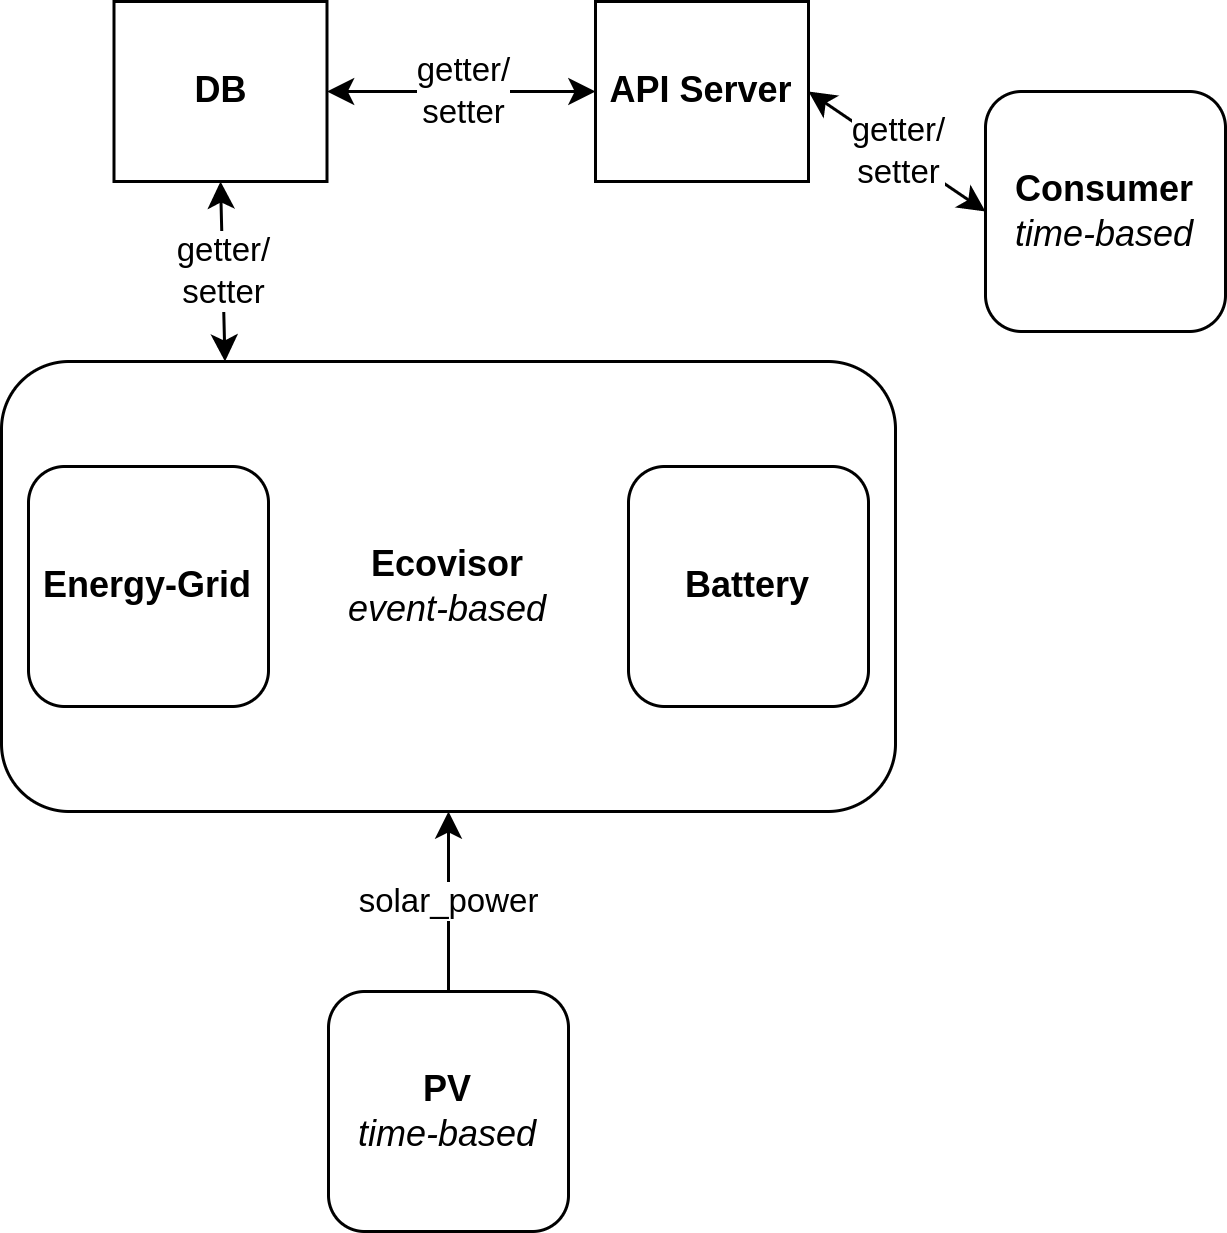
\includegraphics[width=.65\textwidth]{sketch}
        \caption{Ecovisor simulated within Mosaik Co-Simulation; adapted from
        Souza et al. \cite{souza2022}}
    \end{minipage}
    \end{figure}
\end{frame}

\section{Research Question}
\begin{frame}
    \begin{itemize}
        \item interconnected geo-distributed Ecovisors
            \begin{itemize}
                \item carbon intensity different from region to region
                \item carbon information services such as Electricity Maps
                    \footnote{\url{https://www.electricitymaps.com/}\vspace{1cm}}
            \end{itemize}
    \end{itemize}
    \vspace{3mm}
    \begin{itemize}
        \item[\MVRightarrow] enable carbon-efficiency optimizations such as
            Let's Wait Awhile or Cucumber from Wiesner et al. \cite{wiesner2021,
            wiesner2022}
    \end{itemize}
\end{frame}

\appendix

\begin{frame}[noframenumbering]
\bibliographystyle{ieeetr}
\bibliography{refs}
\end{frame}

\end{document}
